
\label{section:switch_small_signal_begin}

\subsection{Análisis de etapa en seguidor por emisor, $Q_{10}$}

\subsubsection{Análisis de la ganancia de tensión}

Dado que este circuito no cumple la condición, $r_{o} \gg R_{E}$ no se puede usar la expresión aproximada $A_{v} \approx \frac{gm \cdot R_{E}}{1 + gm \cdot R_{E}}$, con lo que tenemos:

\begin{equation}
A_{v_{Q_{10}}} = \frac{1}{1 + \frac{r_{\pi_{10}}}{  \left(  \beta_{10} + 1 \right) \cdot \left(  R_{i_{B_{Q_{9}}}} \parallelresistors r_{o_{10}}  \right)  } }
\end{equation}

\begin{equation*}
A_{v_{Q_{10}}} = \frac{1}{1 + \frac{10.1 \si[per-mode=symbol]{\kilo\ohm}}{  \left(  324 + 1 \right) \cdot \left(  1.47 \si[per-mode=symbol]{\mega\ohm} \parallelresistors 50.9 \si[per-mode=symbol]{\kilo\ohm}  \right)  } } = 0.999
\end{equation*}


\subsubsection{Análisis de la resistencia de entrada}

Para calcular la  resistencia de entrada, vemos que no se cumple la condición $r_{o} \gg R_{E}$, con lo que la expresión aproximada, $ R_{i_{B_{Q_{3}}}} \approx r_{\pi_{3}} + \beta_{3} \cdot R_{E}$ no se puede usar.\\ \\

Tenemos entonces:

\begin{equation}
R_{i_{seguidor_{Q_{10}}}} = R_{i_{B_{Q_{10}}}} = r_{\pi_{10}} + \left( \beta_{10} + 1 \right) \cdot  \left(  R_{i_{seguidor_{Q_{9}}}} \parallelresistors R_{22}   \right)  \cdot \frac{  r_{o_{10}} }{  r_{o_{10}} + \left(  1.47 \si[per-mode=symbol]{\mega\ohm} \parallelresistors R_{22}   \right)  }
\end{equation}


\begin{equation*}
R_{i_{seguidor_{Q_{10}}}} = R_{i_{B_{Q_{10}}}} = 10.1 \si[per-mode=symbol]{\kilo\ohm} + \left( 324 + 1 \right) \cdot  \left(  R_{i_{seguidor_{Q_{9}}}} \parallelresistors 10 \si[per-mode=symbol]{\kilo\ohm}   \right)  \cdot \frac{  50.9 \si[per-mode=symbol]{\kilo\ohm} }{  50.9 \si[per-mode=symbol]{\kilo\ohm} + \left(  1.47 \si[per-mode=symbol]{\mega\ohm} \parallelresistors 10 \si[per-mode=symbol]{\kilo\ohm}   \right)  } = 2.7 \si[per-mode=symbol]{\mega\ohm}
\end{equation*}


\subsubsection{Análisis de la resistencia de salida}

\begin{equation}
R_{o_{seguidor_{Q_{10}}}} = r_{d_{10}} + \frac{   R_{10} \parallelresistors \left( R_{9} + \left[  R_{L} \parallelresistors \left( R_{S} + R_{o_{Sziklai}} \right) \right]  \right) }{\beta_{10}}  
\end{equation}


\begin{equation*}
R_{o_{seguidor_{Q_{10}}}} = 31.25 \si[per-mode=symbol]{\ohm} + \frac{   10 \si[per-mode=symbol]{\kilo\ohm} \parallelresistors \left( 10 \si[per-mode=symbol]{\kilo\ohm} + \left[  100 \si[per-mode=symbol]{\ohm} \parallelresistors \left( 0.2 \si[per-mode=symbol]{\ohm} + 114.11 \si[per-mode=symbol]{\milli\ohm} \right) \right]  \right) }{324} = 46.68 \si[per-mode=symbol]{\ohm}
\end{equation*}


\subsection{Análisis de etapa en seguidor por emisor, $Q_{9}$}



\subsubsection{Análisis de la ganancia de tensión}

\begin{equation}
A_{v_{Q_{9}}} = \frac{1}{1 + \frac{r_{\pi_{9}}}{  \left(  \beta_{9} + 1 \right) \cdot \left(  R_{23} \parallelresistors \left(  R_{7} + r_{\pi_{12}} \right) \parallelresistors r_{o_{9}}  \right)  } }
\end{equation}


\begin{equation*}
A_{v_{Q_{9}}} = \frac{1}{1 + \frac{ 14.5 \si[per-mode=symbol]{\kilo\ohm} }{  \left(  335 + 1 \right) \cdot \left(  10 \si[per-mode=symbol]{\kilo\ohm} \parallelresistors \left(  1 \si[per-mode=symbol]{\kilo\ohm} + 7.21 \si[per-mode=symbol]{\kilo\ohm} \right) \parallelresistors 117 \si[per-mode=symbol]{\kilo\ohm}  \right)  } } = 0.99
\end{equation*}


\subsubsection{Análisis de la resistencia de entrada}

\begin{equation}
R_{i_{seguidor_{Q_{9}}}} = R_{i_{B_{Q_{9}}}} = r_{\pi_{9}} + \left( \beta_{9} + 1 \right) \cdot  \left[  R_{23} \parallelresistors \left(  R_{7} + r_{\pi_{12}} \right)   \right]  \cdot \frac{  r_{o_{9}} }{  r_{o_{9}} + \left[  R_{23} \parallelresistors \left(  R_{7} + r_{\pi_{12}} \right)   \right]  }
\end{equation}


\begin{equation*}
R_{i_{seguidor_{Q_{9}}}} = R_{i_{B_{Q_{9}}}} = 14.5 \si[per-mode=symbol]{\kilo\ohm} + \left( 335 + 1 \right) \cdot  \left[  10 \si[per-mode=symbol]{\kilo\ohm} \parallelresistors \left(  1 \si[per-mode=symbol]{\kilo\ohm} + 7.21 \si[per-mode=symbol]{\kilo\ohm} \right)   \right]  \cdot \frac{  117 \si[per-mode=symbol]{\kilo\ohm} }{  117 \si[per-mode=symbol]{\kilo\ohm} + \left[  10 \si[per-mode=symbol]{\kilo\ohm} \parallelresistors \left(  1 \si[per-mode=symbol]{\kilo\ohm} + 7.21 \si[per-mode=symbol]{\kilo\ohm} \right)   \right]  } = 1.47 \si[per-mode=symbol]{\mega\ohm}
\end{equation*}

\subsubsection{Análisis de la resistencia de salida}

\begin{equation}
R_{o_{seguidor_{Q_{9}}}} = r_{d_{9}} + \frac{R_{o_{seguidor_{Q_{10}}}}}{\beta_{9}}  
\end{equation}

\begin{equation*}
R_{o_{seguidor_{Q_{9}}}} = 43.10 \si[per-mode=symbol]{\ohm} + \frac{46.68 \si[per-mode=symbol]{\ohm}}{335} = 43.24 \si[per-mode=symbol]{\ohm} 
\end{equation*}



\label{section:switch_small_signal_end}


\subsection{Análisis del divisor resistivo de realimentación $R_{9}/R_{10}$}

Dado el valor de $R_{i_{seguidor_{Q_{10}}}} = 2.7 \si[per-mode=symbol]{\mega\ohm}$, y el valor de $R_{9}$ y $R_{10}$, se puede asumir que el mismo no está cargado, por lo que su transferencia, será entonces:

\begin{equation}
T_{D_{R_{9}-R_{10}}} = \frac{R_{10}}{R_{9} + R_{10}}
\end{equation}



\subsection{Transferencia del realimentador}

Dado que el divisor resistivo tiene su transferencia ideal al no estar cargado, tenemos en el camino de realimentación de tensión solo este divisor y la ganancia en cascada de ambos seguidores, la llamamos ganancia de la llave, cuyo valor es:


\begin{equation}
A_{v_{llave}} = A_{v_{Q_{10}}} \cdot A_{v_{Q_{9}}}
\end{equation}

\begin{equation*}
A_{v_{llave}} = 0.999 \times 0.99 \approx 0.99
\end{equation*}


La resistencia de salida de la llave, será la vista hacia la salida del seguidor basado en $Q_{9}$, la misma se ve en paralelo con $R_{23}$, tenemos entonces:

\begin{equation}
R_{o_{llave}} = R_{o_{seguidor_{Q_{9}}}} \parallelresistors R_{23}
\end{equation}

\begin{equation*}
R_{o_{llave}} = 43.24 \si[per-mode=symbol]{\ohm} \parallelresistors 10 \si[per-mode=symbol]{\kilo\ohm} = 43.05 \si[per-mode=symbol]{\ohm}
\end{equation*}


\subsection{Cálculo de la ganancia de lazo para el lazo de tensión}

\label{section:voltage_loop_justification}


En la figura~\figref{fig:fig_voltage_loop_1}, puede verse el esquema de la fuente de alimentación como circuito realimentado, puede verse que se trata de realimentación \textbf{serie-paralelo}, que como es de esperarse estabiliza la ganancia de tensión.

\begin{figure}[H] %htb
\begin{center}
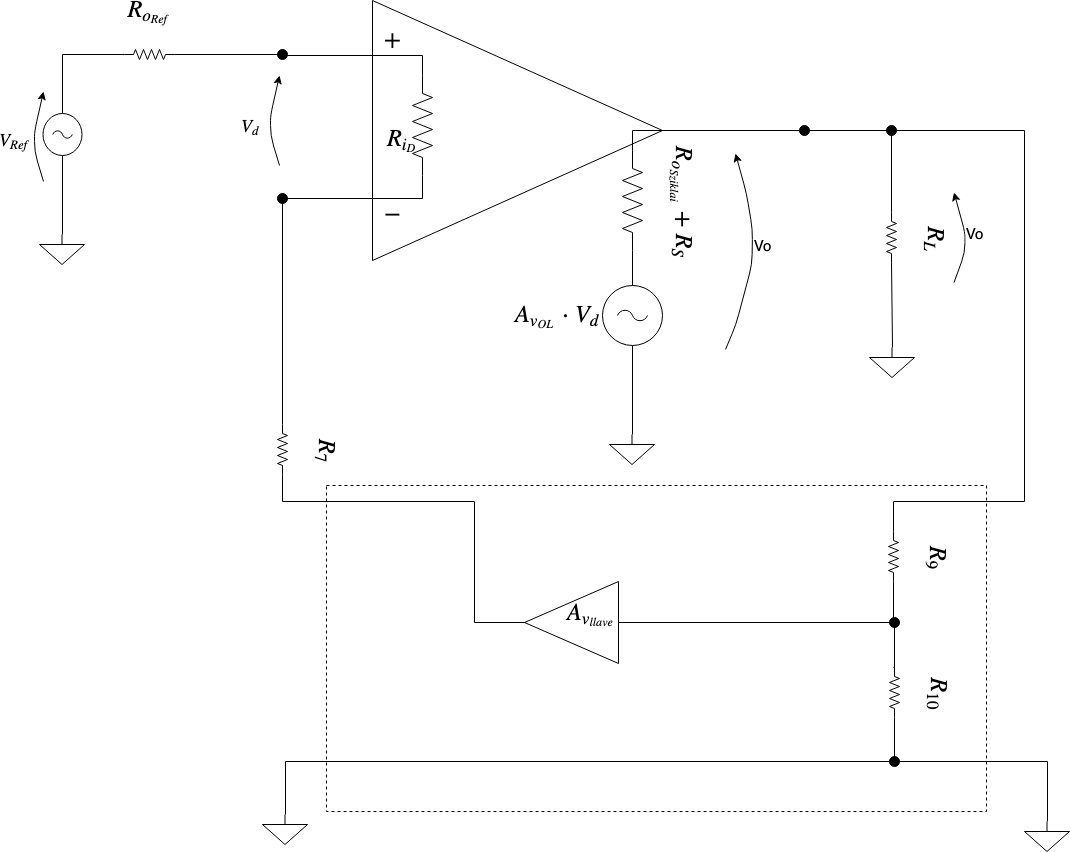
\includegraphics[width=0.9 \textwidth, angle=0]{./img/voltage_loop/VOLTAGE_LOOP_1.png}
\caption{\label{fig:fig_voltage_loop_1}\footnotesize{Esquema de la fuente de alimentación como circuito realimentado}}
\end{center}
\end{figure}

Aplicando parámetros \textbf{h} al realimentador, y reordenando el circuito para llevar el realimentador a su forma ideal, se obtiene lo que se muestra en la figura~\figref{fig:fig_voltage_loop_2}


\begin{figure}[H] %htb
\begin{center}
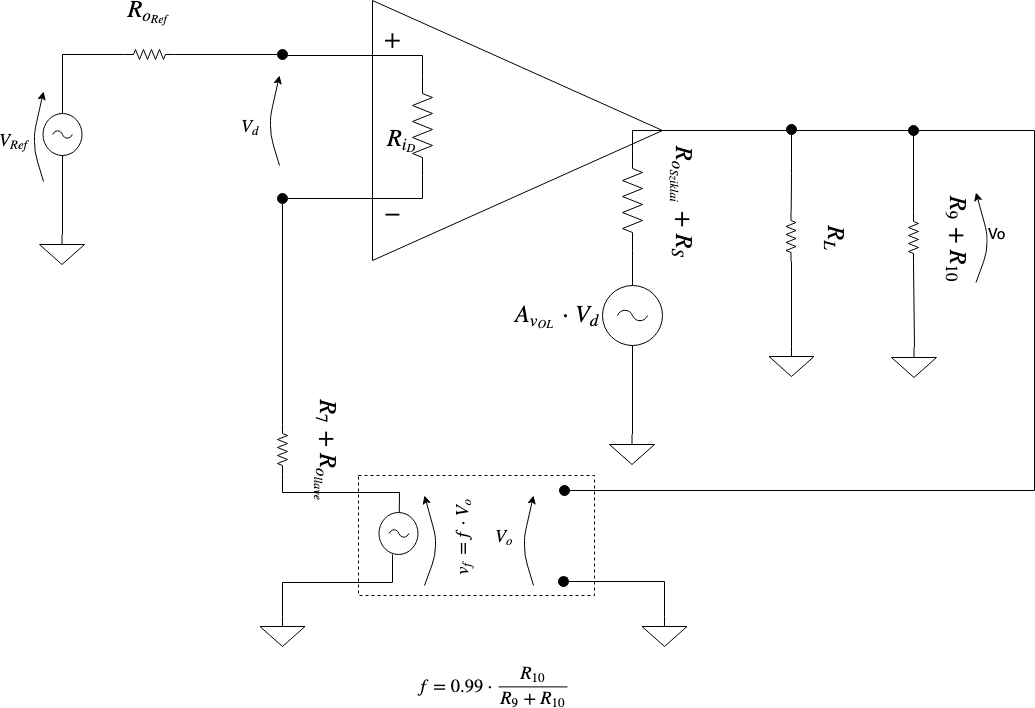
\includegraphics[width=0.9 \textwidth, angle=0]{./img/voltage_loop/VOLTAGE_LOOP_2.png}
\caption{\label{fig:fig_voltage_loop_2}\footnotesize{Aplicando parámetros \textbf{h} al realimentador}}
\end{center}
\end{figure}

\begin{equation}
f = 0.99 \times \frac{R_{10}}{R{9} + R{10}}
\end{equation}


\begin{equation}
a = \evalat{\frac{V_{o}}{V_{Ref}}}{f=0} = \frac{  R_{i_{D}} }{ R_{i_{D}} + R_{7} + R_{o_{llave}} + R_{o_{Ref}}  } \cdot A{v_{OL}} \cdot \frac{  R_{L} \parallelresistors \left( R_{9} + R_{10} \right)  }{ R_{L} \parallelresistors \left( R_{9} + R_{10} \right) + R_{S} + R_{o_{Sziklai}} }
\end{equation}


\begin{equation*}
a = \frac{  15.34 \si[per-mode=symbol]{\kilo\ohm} }{ 15.34 \si[per-mode=symbol]{\kilo\ohm} + 1 \si[per-mode=symbol]{\kilo\ohm} + 43.05 \si[per-mode=symbol]{\ohm} + 1 \si[per-mode=symbol]{\kilo\ohm}  } \times 2382.03 \times \frac{ 100 \si[per-mode=symbol]{\ohm} \parallelresistors \left( 10 \si[per-mode=symbol]{\kilo\ohm} + 10 \si[per-mode=symbol]{\kilo\ohm} \right)  }{100 \si[per-mode=symbol]{\ohm} \parallelresistors \left( 10 \si[per-mode=symbol]{\kilo\ohm} + 10 \si[per-mode=symbol]{\kilo\ohm} \right) + 0.2 \si[per-mode=symbol]{\ohm} + 171.14 \si[per-mode=symbol]{\milli\ohm} } = 2094.26
\end{equation*}



Finalmente tenemos para la ganancia de tensión a lazo cerrado:


\begin{equation}
A = \frac{a}{1 + a \cdot f}
\end{equation}

\begin{equation*}
\boxed{ A = \frac{2094.26}{1 + 2094.26 \times 0.99 \times \frac{R_{10}}{R{9} + R{10}}} \approx 1.01 \times \left(  1 + \frac{R_{9}}{R{10}} \right) }
\end{equation*}

\subsection{Cálculo de la tensión de salida a lazo cerrado}


Para la tensión de salida, asumiendo una tensión de referencia de exactamente $1 \si[per-mode=symbol]{\volt}$:

\begin{equation*}
\boxed{ V{o} = A \cdot V_{Ref} = 1.01 \si[per-mode=symbol]{\volt} \times \left(  1 + \frac{R_{9}}{R{10}} \right) }
\end{equation*}



\subsection{Cálculo de la resistencia de salida a lazo abierto}


La resistencia de la fuente en el nodo de salida a lazo abierto será:

\begin{equation}
R_{o_{OL}} \approx R_{o_{Sziklai}} + R_{S}
\end{equation}


\subsection{Cálculo de la resistencia de salida a lazo cerrado}


Se tendrá entonces a lazo cerrado:

\begin{equation}
R_{o} =  \frac{R_{o_{Sziklai}} + R_{S}}{1 + a \cdot f} 
\end{equation}


\begin{equation}
\boxed{R_{o} = \frac{114.11 \si[per-mode=symbol]{\milli\ohm} + 0.2 \si[per-mode=symbol]{\ohm}}{1 + 2094.263 \times 0.99 \times \frac{R_{10}}{R{9} + R{10}}} = \frac{314.11 \si[per-mode=symbol]{\milli\ohm}}{1 + 2094.26 \times \frac{R_{10}}{R{9} + R_{10}}} \approx 150 \si[per-mode=symbol]{\micro\ohm} \times \left(  1 + \frac{R_{9}}{R{10}} \right) }
\end{equation}

El valor de la misma depende de la realimentación como era de esperar, (también de la ganancia de lazo, esta no es estabilizada). Para el caso de $R_{9} = 10 \si[per-mode=symbol]{\kilo\ohm}$ tenemos:

\begin{equation*}
R_{o_{\left( R_{9} = 10 \si[per-mode=symbol]{\kilo\ohm} \right)}} = 300 \si[per-mode=symbol]{\micro\ohm}
\end{equation*}






